% !TeX root = main.tex
\lecture{17}{Tue 17 Mar 2026 12:00}{Statistical Physics IV: Boltzmann Factors and Degeneracies}

Recap from last lecture:

\begin{itemize}
    \item We can predict the microscopic behaviour of a system using a probability density function defined using macroscopic terms.
    \item We can predict the likelihood of a given energy state begin populated for a system (discrete or continuous) with the Boltzmann factor.
    \item For a two level system with $E_1 < E_0$ we have:
    \[
        Pr\left(E_i\right) = \frac{\exp\left(\frac{-E_i}{k_B T}\right)}{\exp\left(\frac{-E_0}{k_B T}\right) + \exp\left(\frac{-E_1}{k_B T}\right)}
    \]
    \item For a system with $N$ levels, we have:
    \[
        Pr\left(E_i\right) = \frac{\exp\left(\frac{-E_i}{k_B T}\right)}{\sum_{j=0}^{N-1} \exp\left(\frac{-E_j}{k_B T}\right)}
    \]
\end{itemize}

\section{Degeneracies}
In an atom, electrons can have the same energy in multiple different combinations (multiple ways of having the same result). For example, considering only one energy level, electrons can be spin up or spin down. This gives two possible options, hence a degeneracy of two.

With electrons in shells, the degeneracy gives the number of electrons which can fit in a shell. The Pauli exclusion principle says that no two atoms can occupy a shell if they share a quantum number, so the number of possible combinations of distinct states is equal to the number of possible electrons in the shell.

Given the degeneracy $g(E)$, we can modify the Boltzmann Factor accordingly:
\[
    \Pr(E_i) \propto g(E) \exp\left(\frac{-E_i}{k_B T}\right)
\]

For $n = 1$, $g(E) = 2$, for $n = 2$, $g(E) = 4$, and so on.

\section{Boltzmann Factors and Ideal Gases}
For an ideal gas, we have some assumptions (in terms of energy) that have been discussed previously. The most important of these in terms of energy is:
\begin{itemize}
    \item Internal energy all comes from the average kinetic energy of the molecules (temperature) and not from potential energy.
    \item The Boltzmann Factor for an ideal gas hence takes the form:
    \[
        \Pr(E_i) \propto \exp\left(\frac{-E_K}{k_B T}\right)
    \]
\end{itemize}

Our other assumptions are:
\begin{enumerate}
    \item The gas is in thermal equilibrium, hence $\langle E_K\rangle$ is constant.
    \item No gravity (as molecules are extremely light).
    \item Assume that the average separation of each molecule is much larger than the molecule size, hence collisions are infrequent.
    \item There is a very large number of molecules $\sim 10^{23}$ to allow us to treat the gas statistically without high statistical uncertainties.
    \item All molecules have the same mass and size. This is not a good assumption for gases made up of multiple component gases mixed.
    \item We assume that the direction of molecular motion is effectively random, i.e. is unbiased to any particular direction.
    \item Molecules can collide, but do so elastically (and as previously mentioned, infrequently).
    \item Molecules are not relativistic, so $E_K = 0.5 mv^2$ holds.
\end{enumerate}

\section{Model of Ideal Gas}
We can split the velocity of a gas into three cartesian coordinates by adding in quadrature:
\[
    v = \sqrt{v_x^2 + v_y^2 + v_x^2}
\]

By assumption 6, we assume that all of these components are effectively equal, so we can consider the x-direction alone initially (and extrapolate out).

We want to consider the probability of having a velocity somewhere between $v_x$ and $v_x + dx$.
\[
    \Pr(v_x \to v_x + dx) = \int_{v_x}^{v_x + dx} \Pr(v+x) \, dv_x
\]
\[
    = \int_{v_x}^{v_x + dx} C \exp\left(- \frac{-0.5 m v_x^2}{k_B T}\right) \, dv_x
\]

And using the standard integral: $\int_{\infty}^{\infty} e^{-ax^2} \, d = \sqrt{\pi / a}$:

%TODO

\subsection{Density of States}
While we had no degeneracies in each component direction, we do have degeneracies for $v$ itself. For example, $v^2 = 100$ could mean that x, y are zero and $z = 10$, or any other number of combinations.

We therefore want to define the degeneracies as a function of $v$. As a model, consider a grid of infinitesimally small dots in 2D (but for the actual application we would want a 3D model). For some radius, we can count the number of dots which are present on the circumference:

%TODO

Applying this to the Maxwell-Boltzmann distribution, we obtain:
\[
    \Pr(v) = 4 \pi \left(\frac{m}{2 \pi k_B T}\right)^{3/2} v^2 \exp\left(- \frac{mv^2}{2 k_B T}\right) \qquad \text{where: } v \neq 0
\]

This finally gives us the Maxwell-Boltzmann distribution we encountered before (although we have derived it for molecules vs moles):
\begin{figure}[H]
    \centering
    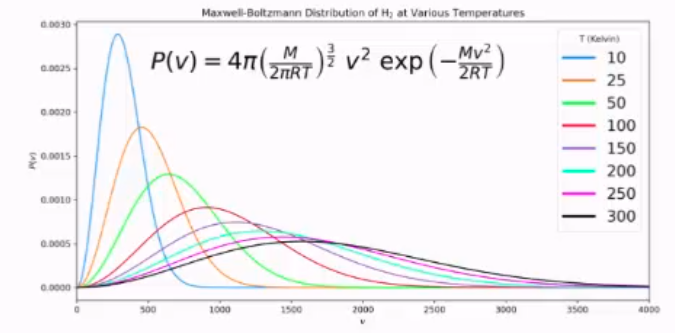
\includegraphics[width=0.75\textwidth]{figures/lec07-1.png}
     \caption{}
\end{figure}

